\documentclass[twocolumn]{IEEEtran}
\usepackage[utf8x]{inputenc}
\usepackage{graphicx}
\usepackage{times}
\usepackage[tbtags]{amsmath}
\usepackage{cite}
%\usepackage{slashbox}
\usepackage{pict2e}
\usepackage{colortbl}
\usepackage{float}
\usepackage[all]{xy}
\usepackage{graphics,graphicx,color,colortbl}
\usepackage{subfigure}
\usepackage{wrapfig}
\usepackage{multicol}
\usepackage{url}
\usepackage[tbtags]{amsmath}
\usepackage{amsmath,amssymb,amsfonts,amsbsy}
\usepackage{bm}
\usepackage{algorithm}
\usepackage{algorithmic}
\usepackage[centerlast, small]{caption}
\usepackage[colorlinks=true, citecolor=blue, linkcolor=blue, urlcolor=blue,
breaklinks=true]{hyperref}
\begin{document}
\title{Proyecto Digital II (AVANCE})
\author{David Ricardo Martínez Hernández Código: $261931$\\
	Juan Sebastian Roncancio Arevalo Código: $261585$}
\maketitle
\markboth{Universidad Nacional de Colombia}{}
\floatname{algorithm}{Algoritmo}
\noindent
A continuación se presentara un avance sobre el proyecto a realizar en la asignatura Electrónica Digital II, el cual tiene como objetivo el control de iluminación y enfocamiento por medio de motores paso a paso, hasta el momento se ha desarrollado bloques de programación para el control de los motores que controlaran la posición de las lámparas; aun no se han probado solo se tienen las estructuras. Estos módulos se han realizado en el lenguaje de descripción de hardware VHDL.\\
Los motores que elegimos para el desarrollo de este proyecto son útiles para la construcción de mecanismos que requieren de bastante precisión,  la característica principal de estos motores es el hecho de poder moverlos un paso a la vez por cada pulso que se le aplique. Este paso puede variar desde 90° hasta pequeños movimientos de tan solo $1.8°$, es decir, que se necesitarán 4 pasos en el primer caso ($90°$) y $200$ para el segundo caso ($1.8°$), para completar un giro completo de $360°$.\\
Para nuestra aplicación no es indispensable la precisión pero por cuestiones de facilidad y presentación decidimos usar estos motores. Cabe aclarar que los motores que usaremos son motores paso a paso bipolares.\\
La corriente necesaria para hacer funcionar los motores es aproximadamente de $2$A, como la FPGA que usaremos no alcanza a proporcionarnos esta corriente hemos decidido usar un circuito conocido como puente H, de este circuito será del que se sacara la corriente para alimentar los circuitos, nosotros usaremos un puente encapsulado comercial con referencia ULN 2803 ya que de los circuitos usados es el que menor número de componentes necesita para funcionar.
\begin{figure}[H]
	\centering
		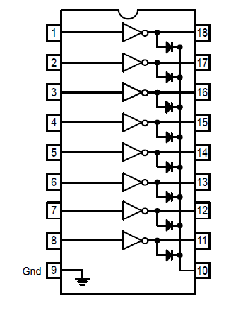
\includegraphics[scale=0.6]{figura1.png}
	\caption{Multiplexor}
	\label{fig1}
\end{figure}
\begin{figure}[H]
	\centering
		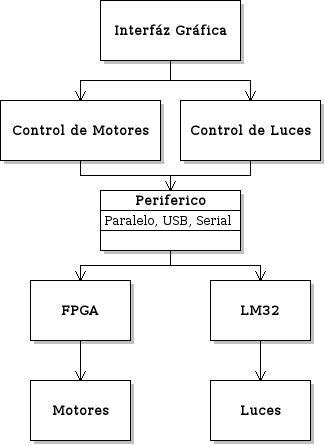
\includegraphics[scale=0.6]{dia1.png}
	\caption{Diagrama de bloques general}
	\label{fig2}
\end{figure}
\noindent
Lo que hasta ahora hemos desarrollado se presenta a continuación en forma de un diagrama de esquemático.
\begin{figure}[H]
	\centering
		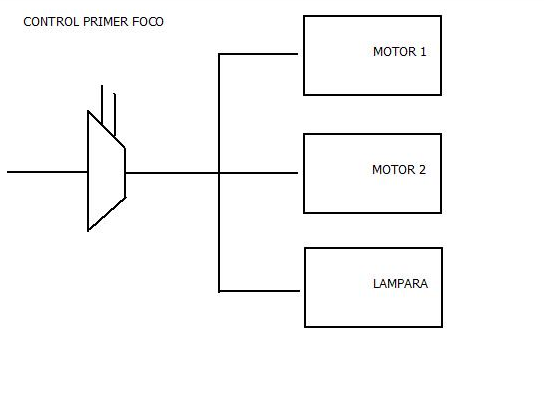
\includegraphics[scale=0.5]{figura2.png}
	\caption{Control de focos y motores}
	\label{fig3}
\end{figure}
\noindent
 Lo que se muestra en la figura \ref{fig3} es la forma en que se controlaran los focos, un foco tiene la forma que se muestra en la figura \ref{fig4}, y está constituido por dos motores paso a paso y una lámpara.\\
El control de los motores se realizara con los módulos escritos en VHDL, y como cada foco tiene dos motores el control del funcionamiento de cada motor se realizara con un switch, es por esta razón que se presenta el multiplexor en la figura \ref{fig3}.
\begin{figure}[H]
	\centering
		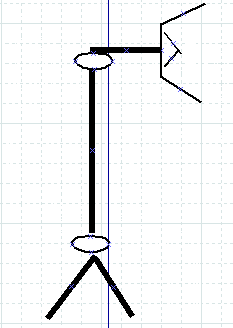
\includegraphics[scale=0.5]{figura3.png}
	\caption{Esquema de la lampara}
	\label{fig4}
\end{figure}
\begin{figure}[H]
	\centering
		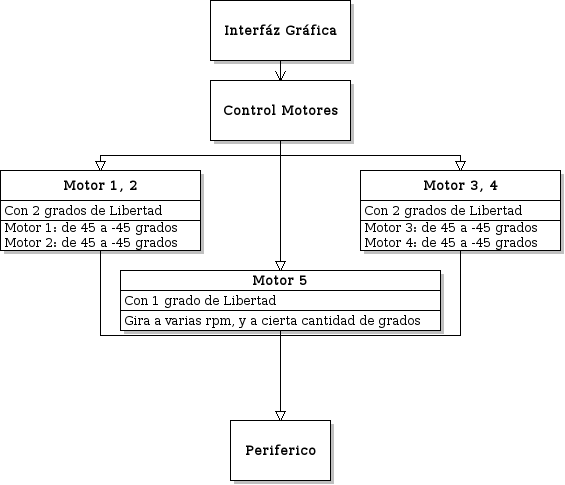
\includegraphics[scale=0.45]{dia2.png}
	\caption{Diagrama de bloques, control de los motores}
	\label{fig5}
\end{figure}
\noindent
Cada lámpara como la que se muestra en la figura \ref{fig4} tiene dos grados de libertad, estos grados de libertad corresponden a los dos óvalos que se ven en la figura y estos óvalos representan cada motor la lámpara puede girar sobre el eje central $180°$, y también puede girar $45°$ para buscar una iluminación centrada en un objeto en especifico.\\
Como se menciono anteriormente también se controlara la iluminación o la intensidad de cada una de las lámparas, esto se realizara con un dimmer. Para estas lámparas se usara una innovación tecnológica que son leds dispuestos en un cinta que se puede moldear hasta encontrar la mejor disposición para así encontrar la mejor iluminación con el menor costo. 
\begin{figure}[H]
	\centering
		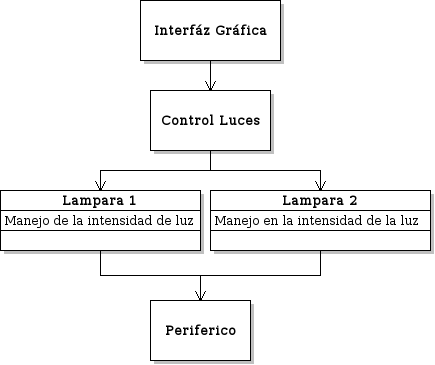
\includegraphics[scale=0.6]{dia3.png}
	\caption{Diagrama de bloques control de luces}
	\label{fig5}
\end{figure}


\bibliographystyle{ieeetran}
\begin{thebibliography}{99}
\bibitem{harris} Harris, David \& Harris, Sarah.
{\em "`Digital desing and computer architecture"'}.
Pretince Hall, 2003.

\bibitem{patterson} Patterson, David \& Hennessy John
{\em "`Computer Organization And Design - The Hardware-Software Interface"'}.
Kindle Edition, Fourth Edition, 2006.

\end{thebibliography}
\end{document}